\documentclass[tikz,border=5pt]{standalone}
\usepackage{times}
\usepackage{amsmath,amssymb}
\usetikzlibrary{positioning,fit,arrows.meta,backgrounds,shapes.geometric,calc,shadows,decorations.pathreplacing}

\begin{document}
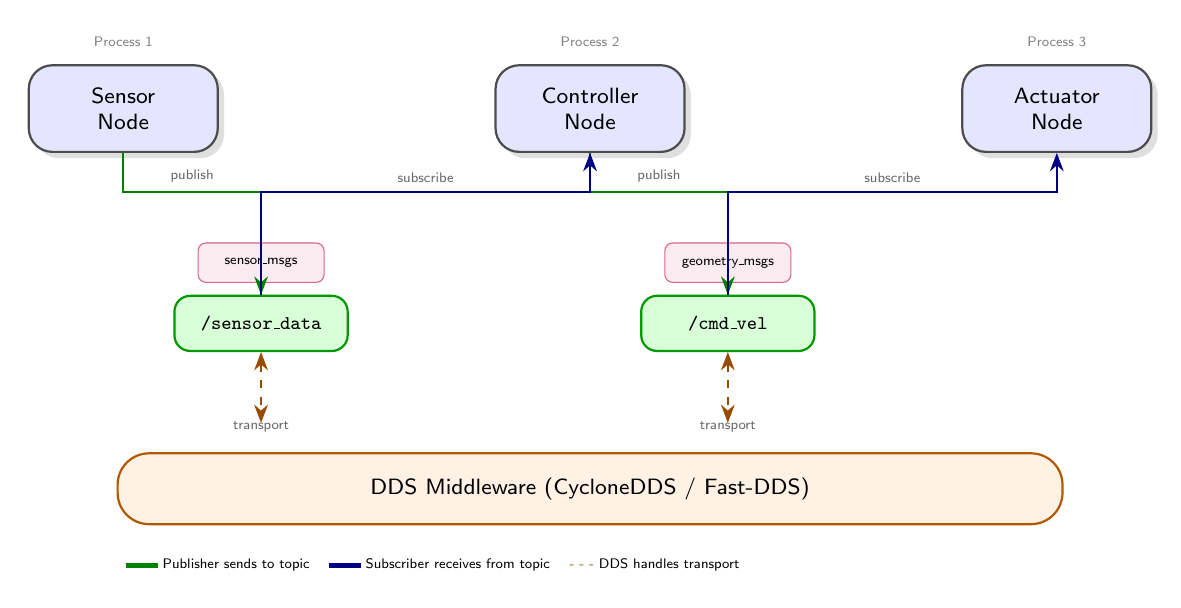
\begin{tikzpicture}[
    node distance=1.2cm and 2.5cm,
    % Node style (ROS 2 computational units)
    rosnode/.style={
        draw=black!70,
        rounded corners=3mm,
        minimum width=2.4cm,
        minimum height=1.1cm,
        font=\sffamily\footnotesize,
        fill=blue!10,
        thick,
        align=center,
        drop shadow={opacity=0.25, shadow xshift=0.08cm, shadow yshift=-0.08cm}
    },
    % Topic style (communication channels)
    topic/.style={
        draw=green!60!black,
        rounded corners=2mm,
        minimum width=2.2cm,
        minimum height=0.7cm,
        font=\sffamily\scriptsize\ttfamily,
        fill=green!15,
        thick,
        align=center
    },
    % DDS layer style
    dds/.style={
        draw=orange!70!black,
        rounded corners=4mm,
        minimum height=0.9cm,
        font=\sffamily\footnotesize,
        fill=orange!10,
        thick,
        align=center
    },
    % Message style
    msg/.style={
        draw=purple!60,
        rounded corners=1mm,
        minimum width=1.6cm,
        minimum height=0.5cm,
        font=\sffamily\tiny,
        fill=purple!8,
        align=center
    },
    % Arrow styles
    pub arrow/.style={->, >=Stealth, thick, color=green!50!black},
    sub arrow/.style={<-, >=Stealth, thick, color=blue!50!black},
    dds arrow/.style={<->, >=Stealth, thick, color=orange!60!black, dashed},
    % Labels
    label/.style={font=\sffamily\tiny, color=black!60}
]

% === ROS 2 Nodes ===
\node[rosnode] (sensor) {Sensor\\Node};
\node[rosnode, right=3.5cm of sensor] (controller) {Controller\\Node};
\node[rosnode, right=3.5cm of controller] (actuator) {Actuator\\Node};

% === Topics (between nodes) ===
\node[topic, below=1.8cm of sensor, xshift=1.75cm] (topic1) {/sensor\_data};
\node[topic, below=1.8cm of controller, xshift=1.75cm] (topic2) {/cmd\_vel};

% === Message types ===
\node[msg, above=0.15cm of topic1] (msg1) {sensor\_msgs};
\node[msg, above=0.15cm of topic2] (msg2) {geometry\_msgs};

% === DDS Layer ===
\node[dds, below=3.8cm of controller, minimum width=12cm] (dds)
    {DDS Middleware (CycloneDDS / Fast-DDS)};

% === Publish arrows ===
\draw[pub arrow] (sensor.south) -- ++(0,-0.5) -| node[label, pos=0.25, above] {publish} (topic1.north);
\draw[pub arrow] (controller.south) -- ++(0,-0.5) -| node[label, pos=0.25, above] {publish} (topic2.north);

% === Subscribe arrows ===
\draw[sub arrow] (controller.south) -- ++(0,-0.5) -| node[label, pos=0.25, above] {subscribe} (topic1.north);
\draw[sub arrow] (actuator.south) -- ++(0,-0.5) -| node[label, pos=0.25, above] {subscribe} (topic2.north);

% === DDS connections ===
\draw[dds arrow] (topic1.south) -- ++(0,-0.6) -- node[label, below, pos=0.5] {transport} ++(0,-0.3);
\draw[dds arrow] (topic2.south) -- ++(0,-0.6) -- node[label, below, pos=0.5] {transport} ++(0,-0.3);

% === Legend ===
\node[below=0.3cm of dds.south west, anchor=north west, font=\sffamily\tiny, align=left] (legend) {
    \textcolor{green!50!black}{\rule{0.4cm}{2pt}} Publisher sends to topic \quad
    \textcolor{blue!50!black}{\rule{0.4cm}{2pt}} Subscriber receives from topic \quad
    \textcolor{orange!60!black}{- - -} DDS handles transport
};

% === Annotations ===
\node[font=\sffamily\tiny, color=black!50, above=0.1cm of sensor.north] {Process 1};
\node[font=\sffamily\tiny, color=black!50, above=0.1cm of controller.north] {Process 2};
\node[font=\sffamily\tiny, color=black!50, above=0.1cm of actuator.north] {Process 3};

\end{tikzpicture}
\end{document}
